\chapter{测试与评估}

本章将介绍面向Hyperledger Fabric的区块链云化框架的测试与评估工作。首先, 本章以典型案例的方式对原型工具进行功能性与非功能性测试;其次, 采用定性与定量方法论\cite{tashakkori1998mixed}结合五层成熟度模型以及与官方工具Cello\footnotemark[1]\footnotetext[1]{\href{https://github.com/hyperledger/cello}{Hyperledger Cello}}进行对比评估。

\section{原型工具测试}

\subsection{测试环境}

为全面对本文提出的区块链云化框架与工具进行测试, 本文对原型工具进行了功能性、非功能性测试以及工具对比测试, 由于在本机环境下搭建Cello会出现诸多问题, 如文件挂载权限、编译等, 所以本文准备了两套测试环境。本文首先在本地环境进行第\ref{section:functional_test}节的功能性测试, 本地机器为MacBook Pro, 并采用Docker for Desktop搭建的单节点Kubernetes充当集群环境; 其次, 在第\ref{section: tool_comparison}节中, 为顺利运行对比工具Cello, 本文利用云主机Ubuntu 18.04搭建Minikube充当集群环境。上述两种环境具体配置如表\ref{computer}所示。

{\footnotesize
\begin{longtable}[h]{m{40pt}|m{100pt}|m{100pt}}
    \caption[配置详情]{配置详情} \label{computer} \\
        \hline   
        \textbf{环境}&\textbf{配置项目}&\textbf{配置详情}\\
        \hline
        \multirow{4}*{\parbox[c]{40pt}{本机环境}}    
        & Docker for Desktop&Version 4.7.0\\     
        & Kubernetes&v1.22.5\\
        & CPU & 4C \\
        & 内存 & 8G \\
        \hline
        \multirow{5}*{\parbox[c]{40pt}{云主机}} 
        & Docker & Community 20.10.13 \\
        & minikube & v1.25.2 \\
        & Kubernetes & v1.23.3 \\
        & CPU & 2C \\
        & 内存 & 4G\\
        \hline 
    \end{longtable} 
}

\subsection{功能性测试}\label{section:functional_test}

本小节主要对原型工具进行功能性测试。如图\ref{fabric_net}所示, 本节将以搭建最经典、简单的HF网络案例的方式进行完整的功能测试。测试重点针对于Ca、Peer、Orderer启动、创建通道、部署链码的全部过程, 验证HF网络启动及链码部署的正确性。

\begin{figure}[h] %figure环境,h默认参数是可以浮动,不是固定在当前位置。如果要不浮动,你就可以使用大写float宏包的H参数,固定图片在当前位置,禁止浮动。
    \centering %使图片居中显示
    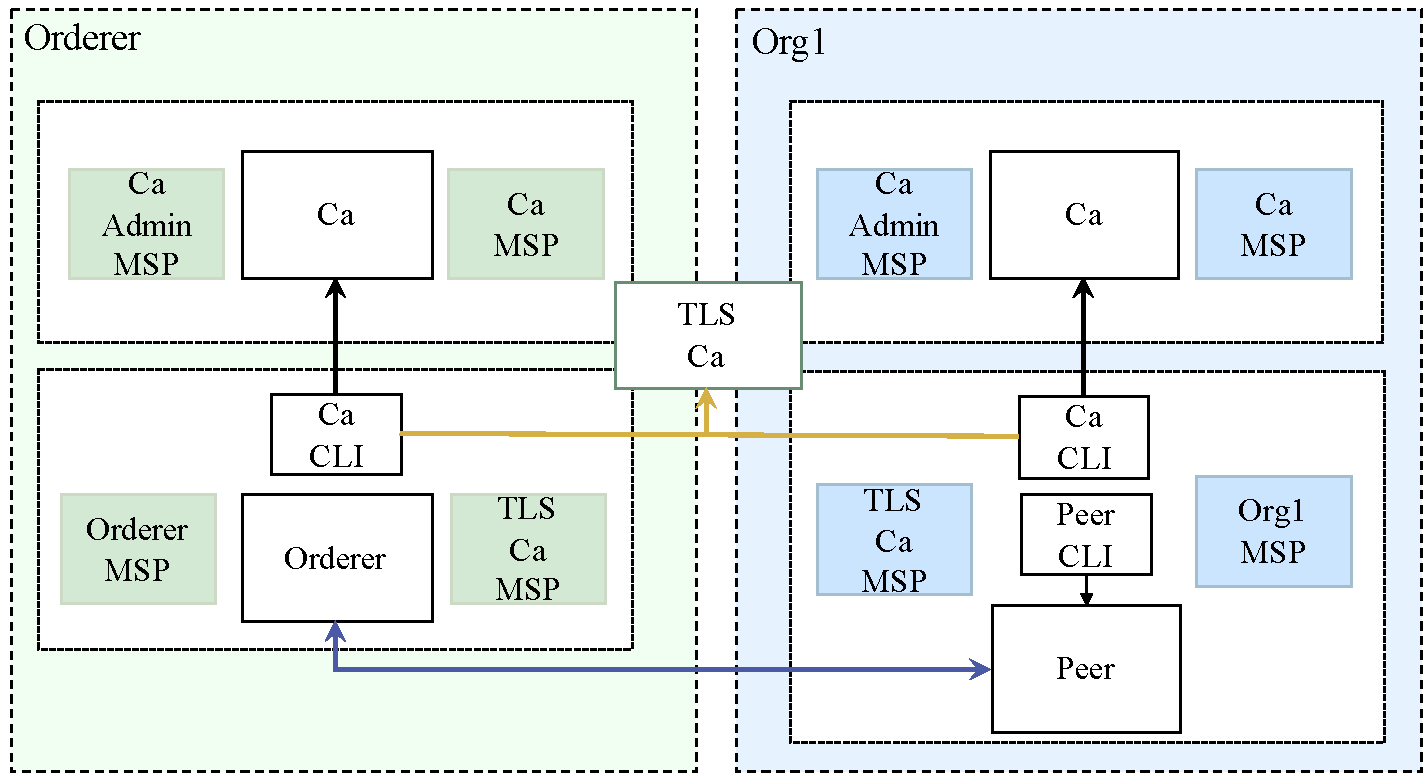
\includegraphics[width=1.0\textwidth]{FIGs/chapter5/fabric_net.pdf} %中括号中的参数是设置图片充满文档的大小,你也可以使用小数来缩小图片的尺寸。
    \caption{测试网络} %caption是用来给图片加上图题的
    \label{fabric_net} %这是添加标签,方便在文章中引用图片。
\end{figure}%figure环境


\textbf{步骤一:} 将原型工具部署入Kubernetes, 原型工具首先将内置的HF网络各节点的CRDs注入Kubernetes。如表\ref{org1_test}所示, HF网络管理员首先为org1创建了名为“org1-ca”的Ca节点; 其次, 在org1中创建了名为“org1-peer0”的Peer节点,并利用链外存储CouchDB作为账本存储单元。如图\ref{testcase1result}所示为测试结果, 原型工具可以为Fabric网络管理员创建Org1的Ca与Peer节点。

{\footnotesize
\begin{longtable}[h]{m{60pt}|m{280pt}}
    \caption[创建Org1测试用例]{Org1测试用例} \label{org1_test}\\
        \hline  
        ID&TC1\\
        \hline
        测试目标&创建含有一个Ca一个Peer的组织Org1\\
        \hline
        前置条件&原型工具已正常启动, Fabric网络各CRDs已经部署进Kubernetes\\
        \hline
        输入& (1)创建Ca节点:“kubectl-hlf ca create --name=org1-ca”
        \newline (2)创建Peer节点:“kubectl-hlf peer create --name=org1-peer0 --mspid=Org1MSP --ca-name=org1-ca.default --db=CouchDB”\\

        \hline 
        预期输出& Org1内包含一个Ca节点以及一个Peer节点\\
        \hline
    \end{longtable} 
}


\begin{figure}[h] %figure环境,h默认参数是可以浮动,不是固定在当前位置。如果要不浮动,你就可以使用大写float宏包的H参数,固定图片在当前位置,禁止浮动。
    \centering %使图片居中显示
    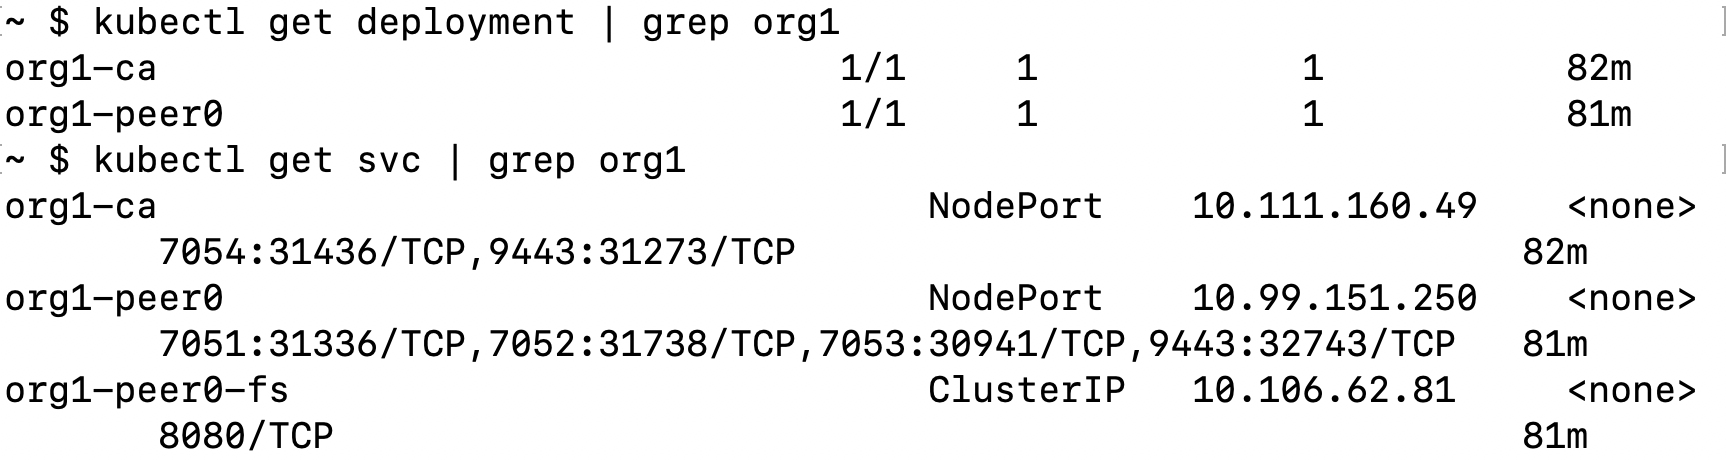
\includegraphics[width=0.9\textwidth]{FIGs/chapter5/peer.png} %中括号中的参数是设置图片充满文档的大小,你也可以使用小数来缩小图片的尺寸。
    \caption{创建Org1测试结果} %caption是用来给图片加上图题的
    \label{testcase1result} %这是添加标签,方便在文章中引用图片。
\end{figure}%figure环境

\textbf{步骤二:} 如表\ref{orderer_test}所示, HF网络管理员需要首先为OrdererMSP创建名为“ord-ca”的Ca节点; 其次, 在OrdererMSP中创建了名为“ord-node1”的Peer节点。如图\ref{testcase2result}所示为测试结果, 原型工具可以为Fabric网络管理员创建Orderer的Ca与Orderer节点, 其中包含但不限于Deployment、Service、Pod、Secret等。

{\footnotesize
\begin{longtable}[h]{m{60pt}|m{280pt}}
    \caption[创建Orderer测试用例]{创建Orderer测试用例} \label{orderer_test}\\
        \hline  
        ID&TC1\\
        \hline
        测试目标&创建含有一个Ca一个Orderer的组织OrdererMSP\\
        \hline
        前置条件&原型工具已正常启动, Fabric网络各CRDs已经部署进Kubernetes\\
        \hline
        输入& (1)创建Ca节点:“kubectl-hlf ca create --name=ord-ca”;
        \newline (2)创建Orderer节点:“kubectl-hlf ordnode create --name=ord-node1 --mspid=OrdererMSP --ca-name=ord-ca.default” \\

        \hline 
        预期输出& OrdererMSP内包含一个Ca节点以及一个Orderer节点\\
        \hline
    \end{longtable} 
}

\begin{figure}[h] %figure环境,h默认参数是可以浮动,不是固定在当前位置。如果要不浮动,你就可以使用大写float宏包的H参数,固定图片在当前位置,禁止浮动。
    \centering %使图片居中显示
    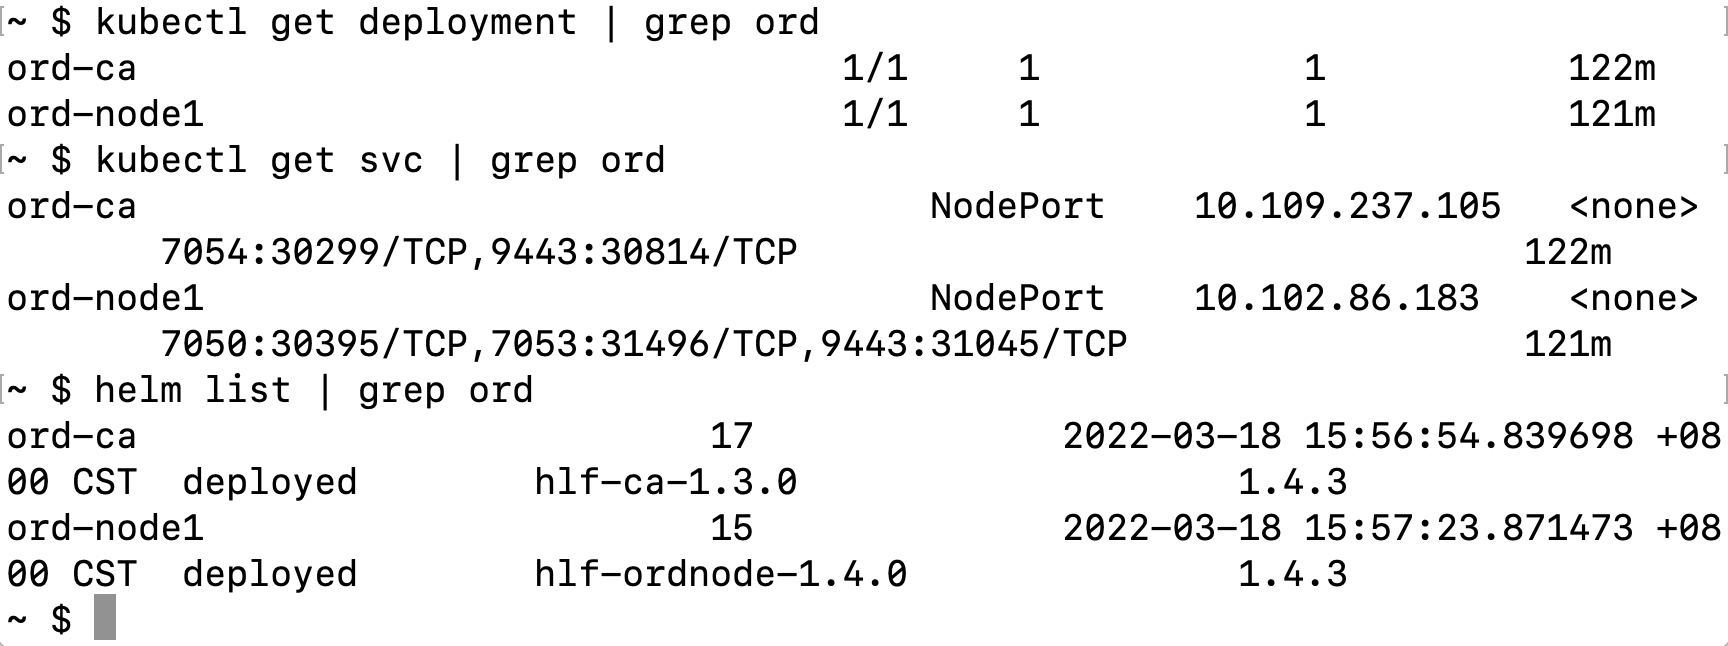
\includegraphics[width=0.9\textwidth]{FIGs/chapter5/orderer.png} %中括号中的参数是设置图片充满文档的大小,你也可以使用小数来缩小图片的尺寸。
    \caption{创建Orderer测试结果} %caption是用来给图片加上图题的
    \label{testcase2result} %这是添加标签,方便在文章中引用图片。
\end{figure}%figure环境

\textbf{步骤三:} 如表\ref{reg_enroll_test}所示, HF网络管理员需要为OrdererMSP以及Org1注册并登记若干用户, 并将用户的证书密钥信息导到yaml文件中。表中仅展示在Orderer中注册用户, Org1中步骤相似(Org1信息输出为org1.yaml)。测试结果表明, 可以成功将用户及OrdererMSP信息导出。

\newpage

{\footnotesize
\begin{longtable}[h]{m{40pt}|m{300pt}}
    \caption[注册、登记用户测试用例]{注册、登记用户测试用例} \label{reg_enroll_test}\\
        \hline  
        ID&TC1\\
        \hline
        测试目标&分别为Orderer以及Org1注册、登记用户\\
        \hline
        前置条件&已经部署完成Orderer、以及Org1中的节点\\
        \hline
        输入& (1)导出Orderer信息:“kubectl-hlf inspect --output=orderer.yaml -o=OrdererMSP”
        \newline (2)注册用户:“kubectl-hlf ca register --name=ord-ca --user=ordereruser --secret=ordererpw --mspid=OrdererMSP”
        \newline (3)登记用户:“kubectl-hlf ca enroll --name=ord-ca --user=ordereruser --secret=ordererpw --mspid=OrdererMSP --output=orderer\_user.yaml”
        \newline (4)加入orderer.yaml:“kubectl-hlf utils adduser --userPath=orderer\_user.yaml --config=orderer.yaml --user=ordereruser --mspid=OrdererMSP”\\

        \hline 
        预期输出& (1)包含ordereruser用户密钥证书信息的orderer\_user.yaml
        \newline (2)包含OrdererMSP所有信息的orderer.yaml\\
        \hline
    \end{longtable} 
}


\textbf{步骤四:} 如表\ref{channel_test}所示, HF开发人员需要在新创建的HF网络上创建通道, 并初始化该通道内的创世区块。当通道被创建完成之后, 需要将在该通道内进行交易的的Orderer、Peer加入该通道。最后, HF开发人员可以指定锚节点并查看通道的高度。如图\ref{channel_test_result}所示为测试结果, 展示了新创建的通道的高度。

{\footnotesize
\begin{longtable}[h]{m{60pt}|m{280pt}}
    \caption[创建通道测试用例]{创建通道测试用例} \label{channel_test}\\
        \hline  
        ID&TC1\\
        \hline
        测试目标&创建通道并将创世节点、org1-peer0加入通道\\
        \hline
        前置条件&已经查创建组织并生成相应用户\\
        \hline
        输入& (1)创建通道:“kubectl-hlf channel generate --output=demo.block --organizations Org1MSP --ordererOrganizations OrdererMSP”
        \newline (2)将Orderer加入通道:“kubectl-hlf ordnode join --name=ord-node1”
        \newline (3)将Peer加入通道:“kubectl-hlf channel join --name=testchannel --user=peeruser --config=org1.yaml -p=org1-peer0”
        \newline (4)检视通道:“kubectl-hlf channel inspect --name=testchannel --user=peeruser --config=org1.yaml -p=org1-peer0 > testchannel.json”
        \newline (5)指定锚节点:“kubectl-hlf channel addanchorpeer --name=testchannel --user=peeruser --config=org1.yaml -p=org1-peer0”
        \newline (6)查看通道高度:“kubectl-hlf channel top --name=testchannel --config=org1.yaml --user=admin -p=org1-peer0”\\

        \hline 
        预期输出& (1)成功创建通道
        \newline (2)成功将创世节点、org1-peer0加入通道
        \newline (3)成功获取通道信息testchannel.json
        \newline (4)成功展示通道高度\\
        \hline
    \end{longtable} 
}

\begin{figure}[h] %figure环境,h默认参数是可以浮动,不是固定在当前位置。如果要不浮动,你就可以使用大写float宏包的H参数,固定图片在当前位置,禁止浮动。
    \centering %使图片居中显示
    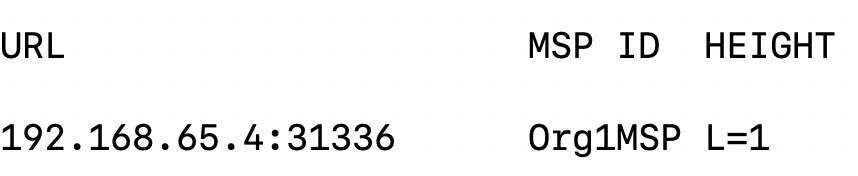
\includegraphics[width=0.55\textwidth]{FIGs/chapter5/channel.png} %中括号中的参数是设置图片充满文档的大小,你也可以使用小数来缩小图片的尺寸。
    \caption{查看通道高度测试结果} %caption是用来给图片加上图题的
    \label{channel_test_result} %这是添加标签,方便在文章中引用图片。
\end{figure}%figure环境

\textbf{步骤五:} 如表\ref{chaincode_test}所示, 为测试通道内所有的参与节点按照链码的合同规则执行, HF开发人员需要在新创建的通道内安装官方提供的asset\footnotemark[1]\footnotetext[1]{\href{https://github.com/hyperledger/fabric-samples/blob/main/asset-transfer-basic/chaincode-go/chaincode/smartcontract.go}{asset链码}}链码, 安装完链码之后, 需要对其进行审批、提交。最后, HF开发人员可以调用链码接口对其进行初始化、查询等一系列操作。如图\ref{chaincode_test_result}所示为测试结果, 展示了查询链码之后的结果。

{\footnotesize
\begin{longtable}[h]{m{60pt}|m{280pt}}
    \caption[链码相关测试用例]{链码相关测试用例} \label{chaincode_test}\\
        \hline  
        ID&TC1\\
        \hline
        测试目标&安装、审批、提交、调用、查询链码\\
        \hline
        前置条件&已经成功启动通道\\
        \hline
        输入& (1)安装链码:“kubectl-hlf chaincode install --path=asset --user=peeruser --config=org1.yaml --language=golang --label=asset --peer=org1-peer0
        \newline (2)查询链码:“kubectl-hlf chaincode queryinstalled --user=peeruser --config=org1.yaml --peer=org1-peer0”
        \newline (3)审批链码:“kubectl-hlf chaincode approveformyorg --user=peeruser --config=org1.yaml --peer=org1-peer0 --package-id=PACKAGEID --name=asset --policy=POLICY --channel=testchannel”
        \newline (4)提交链码:“kubectl-hlf chaincode commit --config=org1.yaml --peer=org1-peer0 --name=asset --policy=\$POLICY --channel=testchannel”
        \newline (5)调用链码:“kubectl-hlf chaincode invoke --config=org1.yaml --peer=org1-peer0 --chaincode=asset --channel=testchannel --function=\$FUNCTION”
        \newline (6)查询链码:“kubectl-hlf chaincode query --config=org1.yaml --peer=org1-peer0 --chaincode=asset --channel=testchannel --function=\$FUNCTION”\\
        \hline 
        预期输出& 成功安装、查询、审批、提交、调用、查询链码\\
        \hline
    \end{longtable} 
}

\begin{figure}[h] %figure环境,h默认参数是可以浮动,不是固定在当前位置。如果要不浮动,你就可以使用大写float宏包的H参数,固定图片在当前位置,禁止浮动。
    \centering %使图片居中显示
    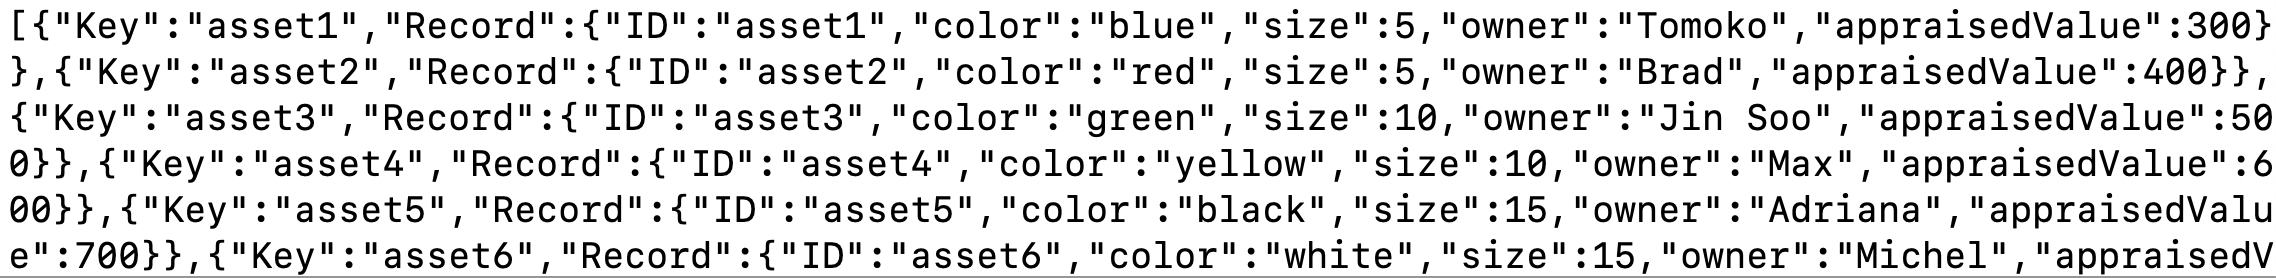
\includegraphics[width=1.0\textwidth]{FIGs/chapter5/chaincode.png} %中括号中的参数是设置图片充满文档的大小,你也可以使用小数来缩小图片的尺寸。
    \caption{查询链码} %caption是用来给图片加上图题的
    \label{chaincode_test_result} %这是添加标签,方便在文章中引用图片。
\end{figure}%figure环境


经过上述步骤1-5, 最终的网络节点状态如图\ref{fabric_result}所示, 本文搭建了一个单Orderer以及单Org、单Peer的简单的Fabric网络, 并分别Orderer、以及Peer搭

\newpage

\noindent
配Ca证书认证。在搭建了基本的网络之后, 分别为Orderer、Peer注册并登记用户, 最后在组织Org中搭建了一个通道并成功安装调用链码。测试结果可知, 本文的原型工具能够正常成功搭建HF网络及部署链码。


\begin{figure}[h] %figure环境,h默认参数是可以浮动,不是固定在当前位置。如果要不浮动,你就可以使用大写float宏包的H参数,固定图片在当前位置,禁止浮动。
    \centering %使图片居中显示
    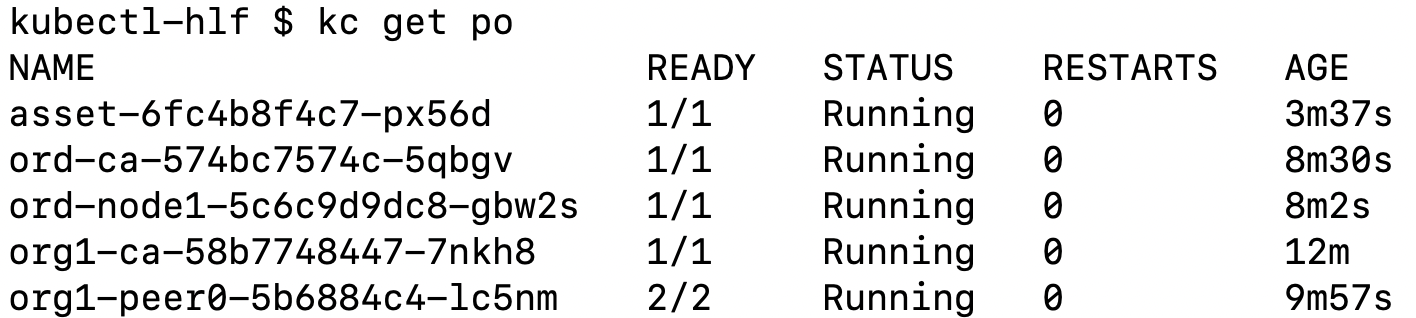
\includegraphics[width=1.0\textwidth]{FIGs/chapter5/fabric_result.png} %中括号中的参数是设置图片充满文档的大小,你也可以使用小数来缩小图片的尺寸。
    \caption{网络节点状态} %caption是用来给图片加上图题的
    \label{fabric_result} %这是添加标签,方便在文章中引用图片。
\end{figure}%figure环境


\subsection{非功能性测试}

本文接下来对原型工具的非功能性需求进行测试, 查看原型工具是否满足第\ref{section: requirement}节所提到的易用性、可扩展性、安全性等非功能性需求。

易用性, 本文邀请了5位熟悉HF基本概念及网络搭建流程的开发人员对本文的原型工具进行易用性测试。为了排除网络的影响,
本文提前下载好原型工具搭建HF网络所需要的Docker镜像。在介绍了本工具的基本原理以及命令行的基本使用方法后, 5位测试的开发人员分别独立自行搭建不同规格的HF网络, 最终5位测试的开发人员都能够在30分钟内学习并掌握原型工具的使用方法。

为测试本工具的可靠性, 本文在使用原型工具搭建HF网络过程中有意输入错误的命令行参数, 输入不正确的密钥文件等, 原型工具都能在1s内给出参数的异常情况; 同时, 原型工具能够有效利用Prometheus监控体系对工具本身以及HF网络的所有节点、智能合约以及DB进行监控, 如图\ref{monitoring}展示了利用Prometheus与Grafana对Fabric Ca Resource进行监控的画面, 图中展示了Fabric Ca Resource的API、内存以及CPU的使用情况。在搭建完HF网络之后, 原型工具在两周内仅崩溃1次, 且能通过日志以及Prometheus的告警设置在5分钟内进行恢复。

为提升原型工具的可迁移性, 本文通过Dockerfile将本工具打包成Docker镜像, 使用预先打包并经过检验的镜像, 并为该原型工具配备专用的Helm chart, 其中包含有关原型工具构建的所有必要信息, 这样可以以最少的时间部署。结果表明, 原型工具可以通过helm在支持Kubernetes 1.18版本以上的云平台上运行, 原型平台具备良好的可迁移性。

\begin{figure}[h] %figure环境,h默认参数是可以浮动,不是固定在当前位置。如果要不浮动,你就可以使用大写float宏包的H参数,固定图片在当前位置,禁止浮动。
    \centering %使图片居中显示
    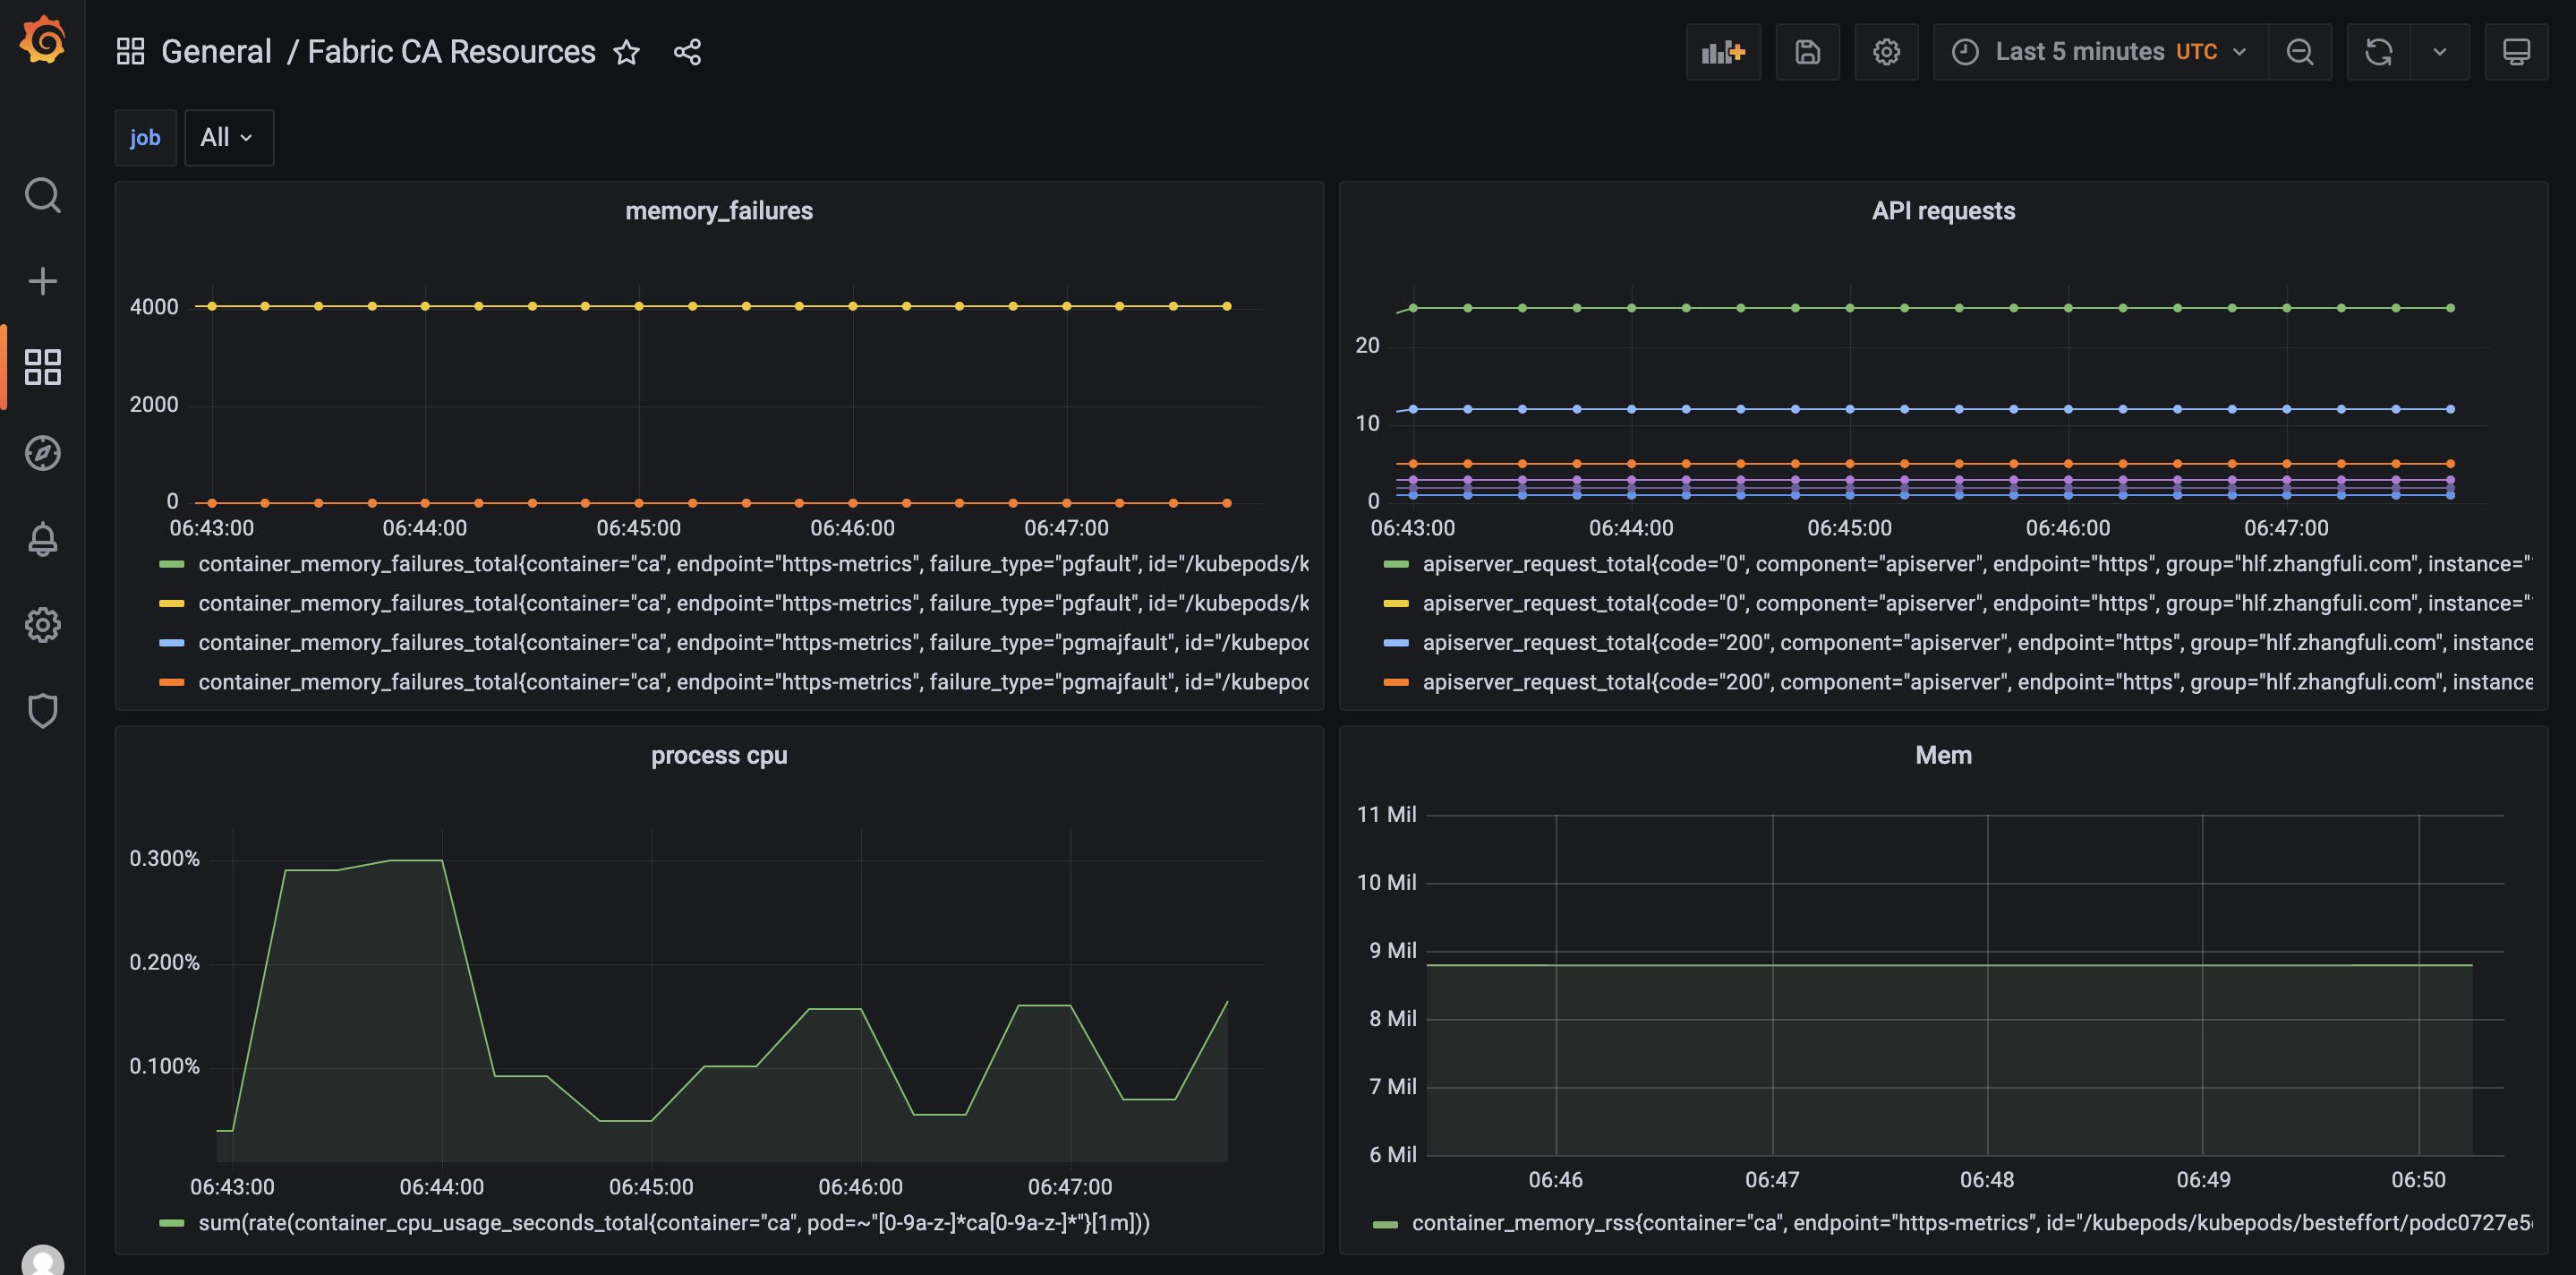
\includegraphics[width=1.0\textwidth]{FIGs/chapter5/monitoring.png} %中括号中的参数是设置图片充满文档的大小,你也可以使用小数来缩小图片的尺寸。
    \caption{Fabric Ca Resource监控图} %caption是用来给图片加上图题的
    \label{monitoring} %这是添加标签,方便在文章中引用图片。
\end{figure}%figure环境

在数据存储及其可扩展性方面, 如图\ref{db}所示, 原型工具为每个HF网络中的工作节点设置了专属存储单元。每个存储单元配置专属的PVC管理, 由于原型工具基础的StorageClass的“allowVolumeExpansion”字段设置为“true”。HF网络管理员可以通过修改已经部署的HF网络节点的CRs进行扩容, 其中可以包含节点资源类型的扩容以及存储单元的扩容。值得注意的是, 由于存储单元PVC扩容依赖于Kubernetes所以当前只有AWS-EBS、GCE-PD、Azure磁盘、Azure文件、Glusterfs、Cinder、Portworx和Ceph RBD数据卷插件才能支撑数据扩容操作。

\begin{figure}[h] %figure环境,h默认参数是可以浮动,不是固定在当前位置。如果要不浮动,你就可以使用大写float宏包的H参数,固定图片在当前位置,禁止浮动。
    \centering %使图片居中显示
    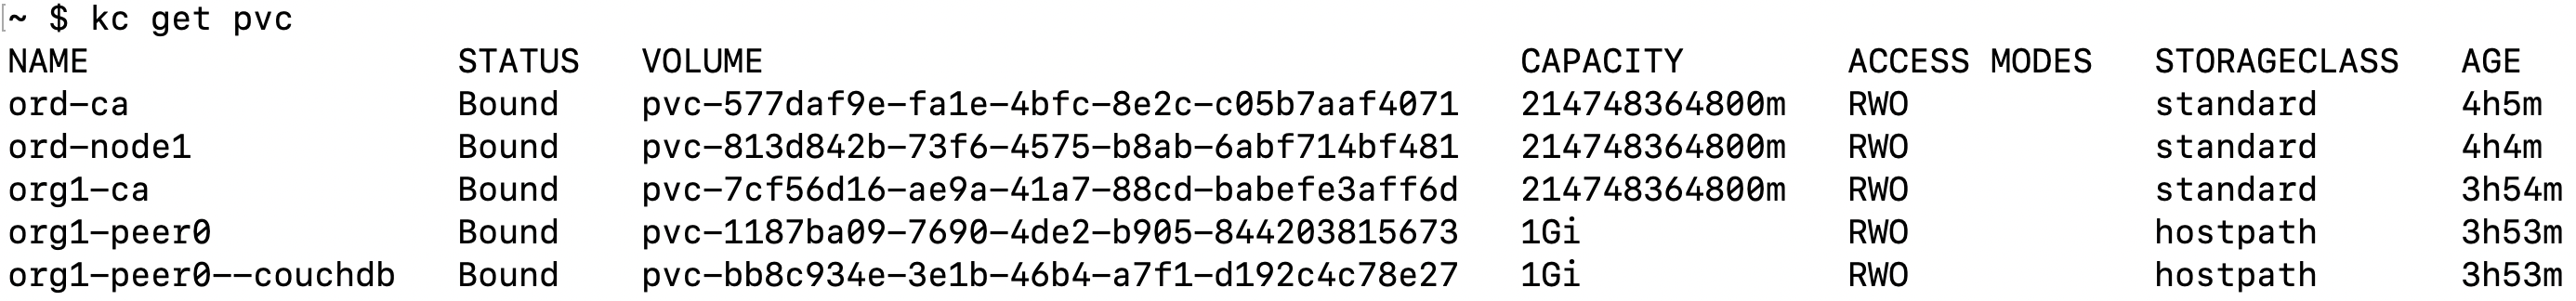
\includegraphics[width=1.0\textwidth]{FIGs/chapter5/db.png} %中括号中的参数是设置图片充满文档的大小,你也可以使用小数来缩小图片的尺寸。
    \caption{网络存储状态} %caption是用来给图片加上图题的
    \label{db} %这是添加标签,方便在文章中引用图片。
\end{figure}%figure环境


在安全性方面, 原型工具具备严格的权限访问控制机制以及密钥保存方式。原型工具将所有的HF资源放在同一命名空间下, 并为该命名空间提供了两种类型的角色。当用户拥有超越权限的操作时, 原型工具会提示并不进行相关操作。同时, 对于生成的HF网络用户而言, 原型工具提供Secret方式为其保存密钥。当这些用户操作HF网络时, 原型工具会要求提供对应的密钥文件作为身份认证的方式。

\section{原型工具评估}

\subsection{五层成熟度模型}

如图所示\ref{maturity}, Kubernetes Operator拥有5个成熟度级别的定义\cite{duan2021case}, 其通过定性的方式分析某个Operator应用是否达到了某个级别, 这5个成熟度级别定义如下:

\begin{itemize}[itemindent=2em]
    \item 第一级: Basic Intall, 该级是Operator成熟度模型中最基本的级别。在该级中, 用户能够使用CRD对目标程序进行配置和安装;

    \item 第二级: Seamless Upgrades, 在该级别上的Operator能够不丢失数据的升级所管理的工作负载;

    \item 第三级: Full Lifecycle, 是否能达到该级别取决于Operator是否具备生命周期管理和的数据备份、恢复能力。在该级别上的Operator能够备份数据, 并在发生任何数据灾难时从备份数据中恢复数据。

    \item 第四级: Deep Insights, Operator提供监控和报警等功能。在该级别, operator能够包含所有组件的运行状况指标, 并根据指标配备报警功能;

    \item 第五级: Auto Pilot, 最终级别拥有许多高级功能, 如自动伸缩。Operator可以通过收集到的指标来扩展工作负载。

\end{itemize}

\begin{figure}[h] %figure环境,h默认参数是可以浮动,不是固定在当前位置。如果要不浮动,你就可以使用大写float宏包的H参数,固定图片在当前位置,禁止浮动。
    \centering %使图片居中显示
    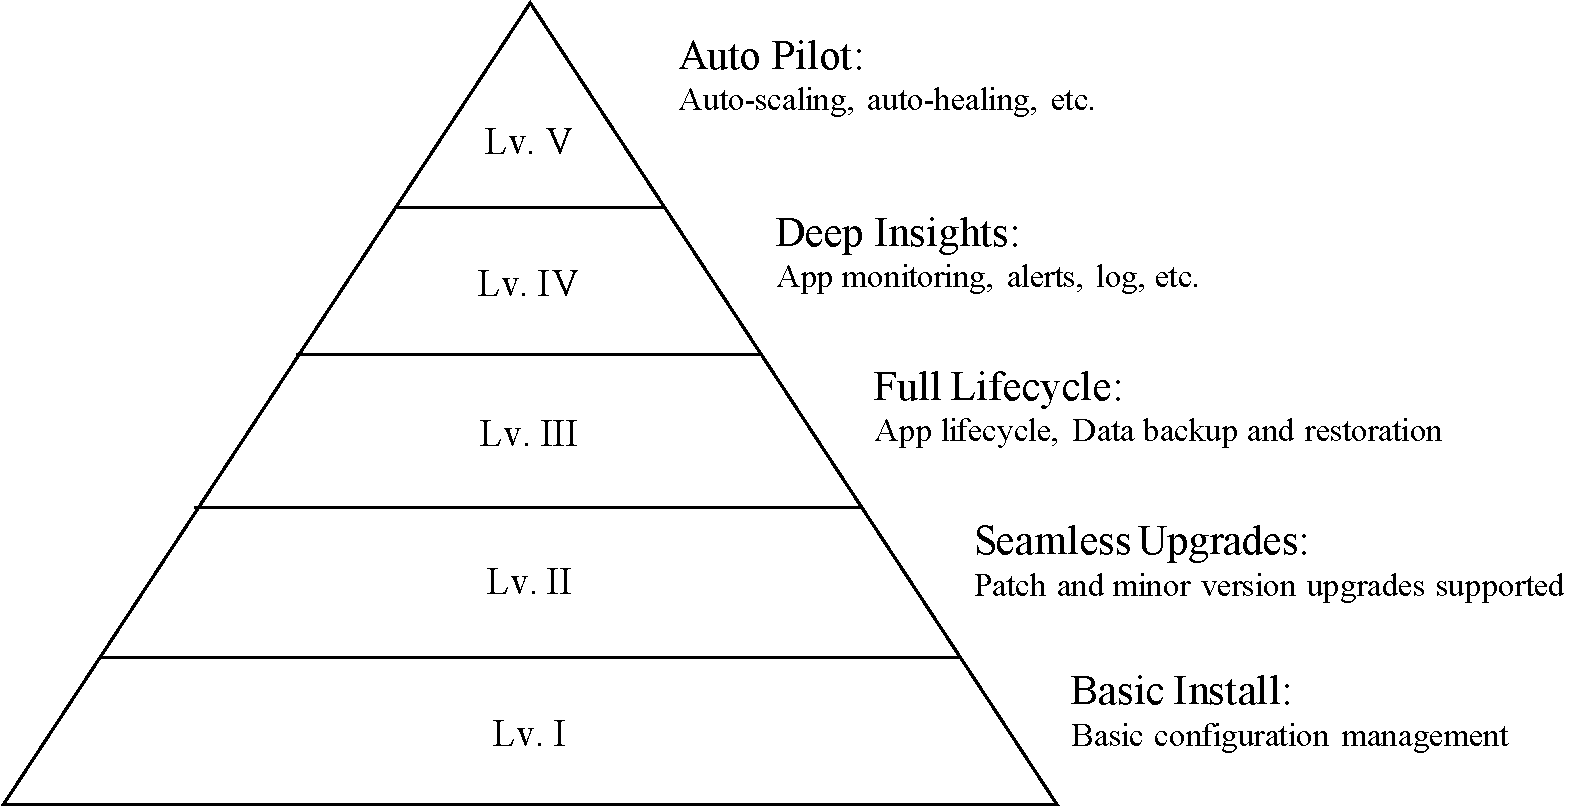
\includegraphics[width=0.9\textwidth]{FIGs/chapter5/maturity.pdf} %中括号中的参数是设置图片充满文档的大小,你也可以使用小数来缩小图片的尺寸。
    \caption{成熟度模型} %caption是用来给图片加上图题的
    \label{maturity} %这是添加标签,方便在文章中引用图片。
\end{figure}%figure环境

\textbf{Basic Install}

借助于原型工具, 能够通过命令行方式一键启停HF网络中任意节点, 而且不需要进行复杂的证书管理。一旦原型工具被部署在Kubernetes网络中, 原型工具就可以对CRs以及Helm进行管理, HF网络管理人员可以借助命令行参数的方式进行创建、更新CRs以此来创建特定规格的HF网络。 一旦CRs进行更新, 原型工具就会将当前状态调整为与指定状态一致。

\textbf{Seamless Upgrades}

在原型工具中, HF网络管理员可以通过修改CRs的内容对包括HF网络节点镜像、端口、host、版本等进行无缝修改。此外, 由于原型工具依赖于链外存储的CouchDB, 以及外部的Prometheus监控体系, 这两者的升级并不会对原型工具产生严重的负面影响。 

\textbf{Full Lifecycle}

虽然原型工具能够在Mangager中对结合Helm对HF网络进行全生命周期管理, 但目前原型工具目前仍缺少数据备份和恢复的能力。要达到这一能力需要在CRs中指定远程备份的数据存储平台, 并在CRs中指定数据备份的凭证以及远程备份的链接。同时, 原型工具在一定的时间周期内将数据备份的到远程的数据存储平台上。

\textbf{Deep Insights}

原型工具利用Prometheus监控体系实现监控与报警的功能, 与此同时, 除了让Prometheus抓取Pod的基本指标外, CRD中还设定了PodMonitor、ServiceMonitor、CouchDBExporter接口, 可以让Prometheus更全面的抓取HF网络的监控指标。HF网络管理员可以通过Grafna可视化图表查看整体HF网络运行状态, 并且能够根据监控指标创建自定义的告警规则。

\textbf{Auto Pilot}

在Kubernetes中存在两种自动伸缩的插件, 即HPA、VPA。当负载超过一定的阈值时, 就会对其进行伸缩或配置更多的资源。然而在HF网络中, 每个Peer都有记录全部账本的职责, 并且只需要超过51\%的Peer节点保持一致即可, 所以针对于Peer并不需要根据监控进行自我伸缩的能力。在数据存储方面, 随着账本的膨胀, 原型工具可以针对链外存储进行扩容。

综上, 通过定性分析, 本文原型工具利用Operator管理Fabric网络能够完美的具备第一级、第二级在第三级上能够支持全生命周期管理但是对于数据的备份能力依旧是存在欠缺, 借助原型工具实现了第四级的监控, 对于自动伸缩方面仅支持数据层面的扩展, 所以本文原型工具基本满足5层成熟度模型的功能。

\subsection{工具对比} \label{section: tool_comparison}

除上述通过定性分析的手段对运行工具进行评估外, 本文选取了Hyperledger官方推出的BaaS平台Cello进行定量数据的对比分析。本文重点关注的是对HF网络节点的云化问题, 所以需要在网络部署时间上对Cello以及原型工具进行对比。

本文在云主机环境下拉取Cello的release-0.9.0-h3c并进行打包构建以及运行。如图\ref{cello}所示, Cello通过图形化的Cello Operator进行主机绑定、组织管理、网络管理以及用户管理。操作Cello Operator的就是HF网络管理员, 管理员首先在主机管理中添加主机, 主机就是Cello将要部署的目标Docker或者Kubernetes环境, 然后再依次创建组织并启动网络, 整个过程全都通过图形化界面的方式完成。

\begin{figure}[h] %figure环境,h默认参数是可以浮动,不是固定在当前位置。如果要不浮动,你就可以使用大写float宏包的H参数,固定图片在当前位置,禁止浮动。
    \centering %使图片居中显示
    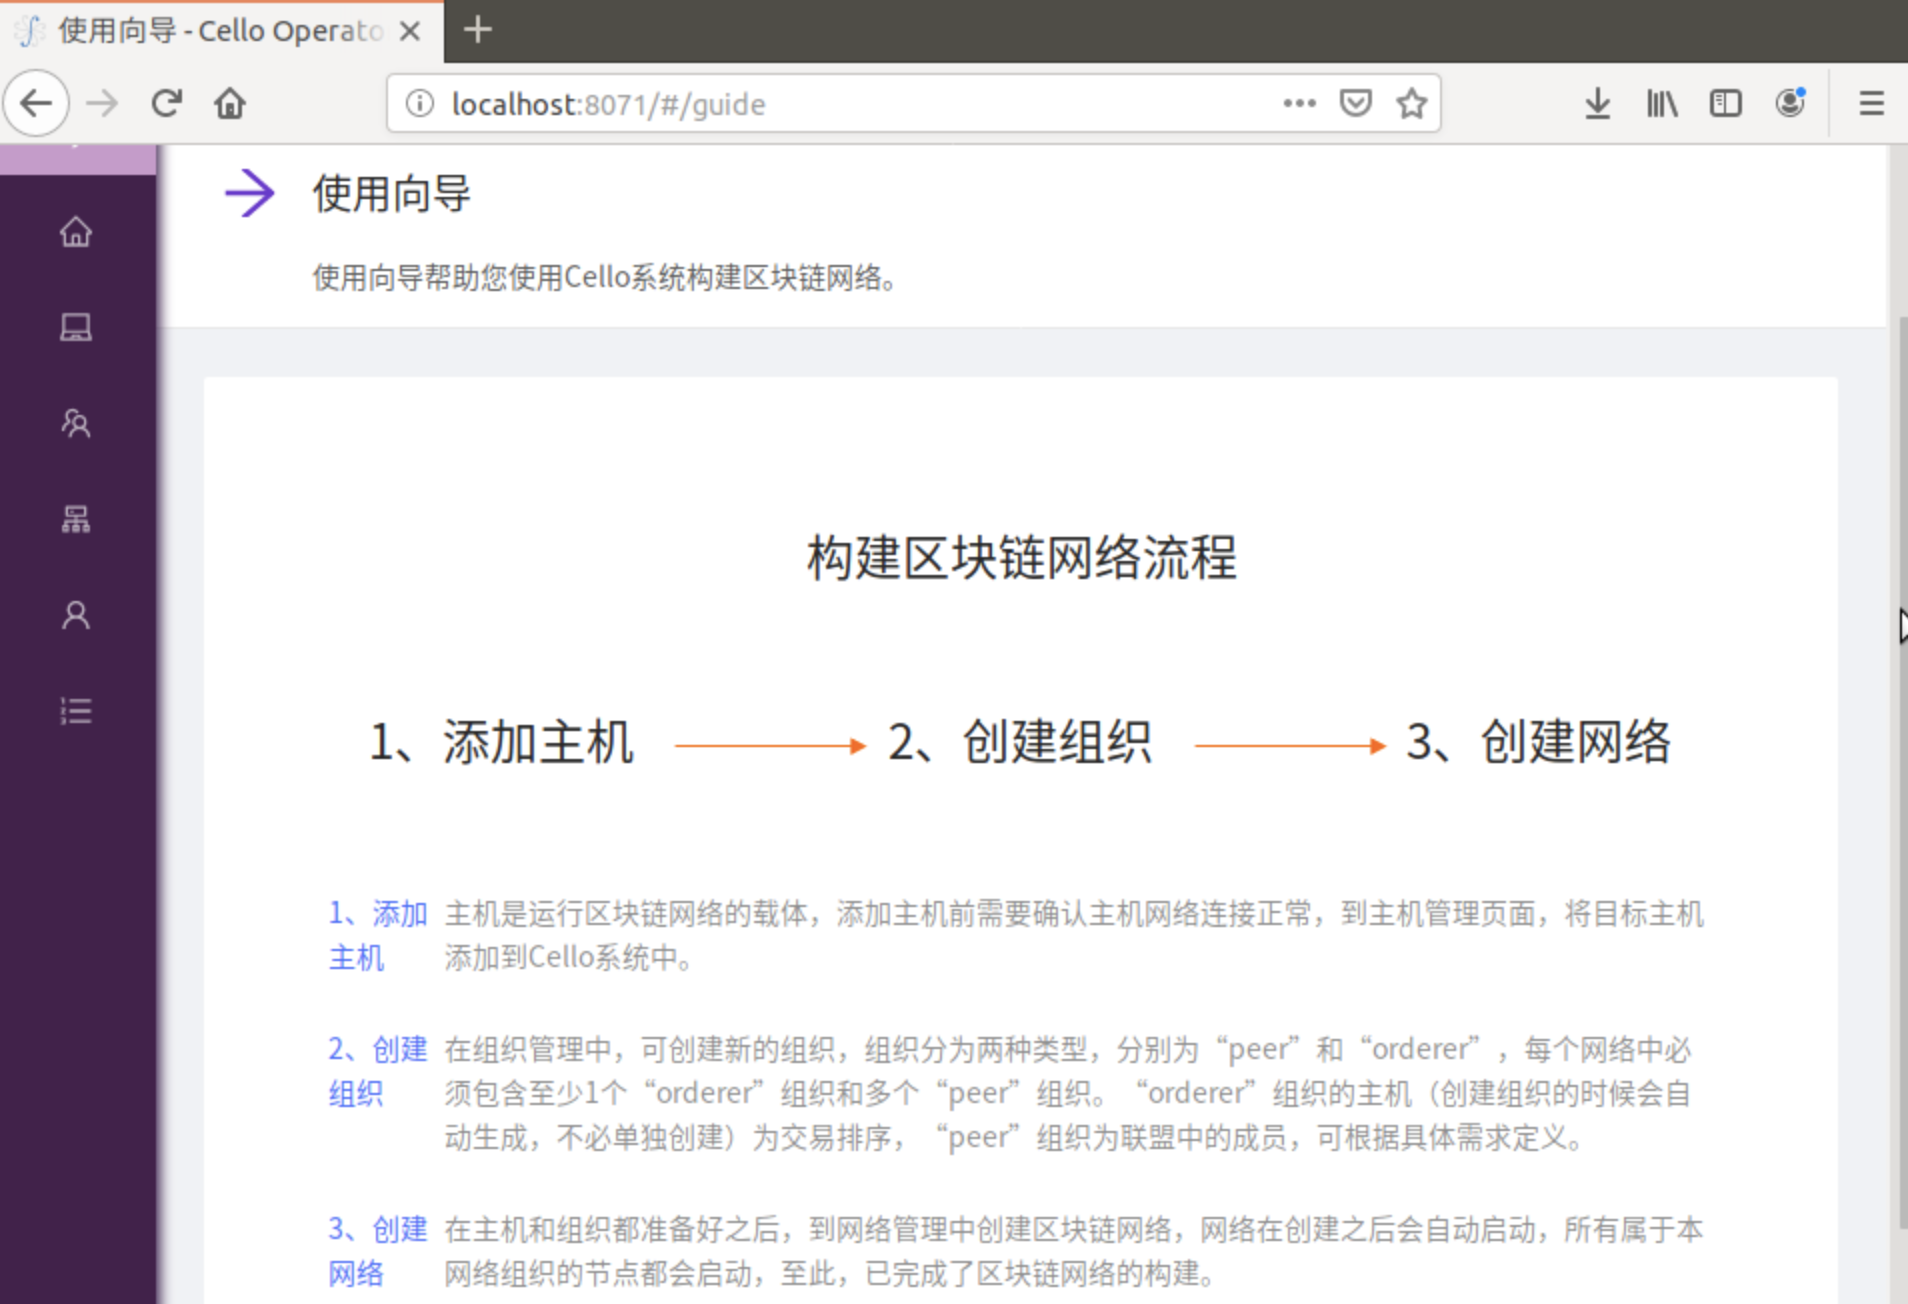
\includegraphics[width=0.95\textwidth]{FIGs/chapter5/cello.png} %中括号中的参数是设置图片充满文档的大小,你也可以使用小数来缩小图片的尺寸。
    \caption{图形化Cello Operator} %caption是用来给图片加上图题的
    \label{cello} %这是添加标签,方便在文章中引用图片。
\end{figure}%figure环境

由于现在在Docker环境中部署HF网络仍旧是主流, 所以本文利用Cello在Docker中部署作为测试基准。由于Cello的局限性, 仅支持在部署HF网络的1.4版本, 而原型工具能更优的支持HF网络的2.X以上版本。
如表\ref{test_fabric_net}展示了本次工具对比所部署的HF网络各节点的版本信息, 测试基准为基于单组织单Peer的网络部署时间, 共识算法选择Solo, 数据存储选择LevelDB。

{\footnotesize
\begin{longtable}[h]{m{50pt} m{100pt} m{50pt}}
    \caption[Hyperledger Fabric版本信息]{Hyperledger Fabric版本信息} \label{test_fabric_net} \\
        \hline  
        \textbf{工具类型}&\textbf{镜像}&\textbf{版本}\\
        \hline
        \multirow{3}*{cello}
        & Fabric-Ca & 1.4.2 \\
        & Fabric-Peer & 1.4.2 \\
        & Fabric-Orderer & 1.4.2 \\
        \hline
        \multirow{3}*{原型工具}
        & Fabric-Ca & 1.4.9 \\
        & Fabric-Peer & 2.4.1 \\
        & Fabric-Orderer & 2.4.1 \\
        \hline
    \end{longtable}
}



为了避免人为的手工干扰, 获得更加准确的网络部署时间。本文提前在Cello Operator中创建好Orderer以及org1组织并为每个组织配置一个对应的节点。当点击提交网络时开始计时, 刚开始创建时, 网络节点的状态是“故障”, 当网络节点的状态从“故障”变成“正常”时停止计时, 随后删除该网络。重复10次上述操作, 且为避免后端镜像遗留干扰, 每次操作间隔3min~5min。在原型工具中, 为避免手工输入命令而带来的人为误差, 本文预先编写好创建网络的的脚本, 脚本中创建10次网络, 创建完成后删除该网络并在删除后休眠30s, 如此循环10次共得到10次网络启动时间如表\ref{net_deployment_time}所示。

{\footnotesize
\begin{longtable}[h]{m{35pt}|m{40pt}|m{15pt} m{15pt} m{15pt} m{15pt} m{15pt} m{15pt} m{15pt} m{15pt} m{15pt} m{15pt}|m{20pt}}
    \caption[网络部署时间(单位: 秒(s))]{网络部署时间(单位: 秒(s))} \label{net_deployment_time}\\
        \hline
        \multirow{2}*{工具类型}
        & \multirow{2}*{\parbox[c]{40pt}{节点类型}}
        & \multicolumn{10}{c|}{序号}
        
        & \multirow{2}*{\parbox[c]{20pt}{平均}}\\
        \cline{3-12}
        & & 1 & 2 & 3 & 4 & 5 & 6 & 7 & 8 & 9 & 10 & \\
        \hline
        cello & 整体网络 & 73 & 119 & 115 & 90 & 73 & 89 & 137 & 85 & 103 & 127 & 101.1\\
        \hline  
        \multirow{5}*{\parbox[c]{40pt}{原型工具}}
        & ca(peer) & 13 & 12 & 13 & 13 & 13 & 13 & 13 & 12 & 12 & 12 & 12.6 \\
        & peer & 20 & 21 & 29 & 16 & 23 & 27 & 20 & 20 & 16 & 22 &  21.4 \\
        & ca(ord) & 13 & 13 & 13 & 13 & 13 & 13 & 14 & 13 & 15 & 15 & 13.5 \\
        & orderer & 27 & 36 & 34 & 24 & 33 & 24 & 27 & 25 & 32 & 25 & 28.7 \\
        \cline{2-13}
        & 整体网络 & 73 & 82 & 89 & 66 & 82 & 77 & 74 & 70 & 75 & 74 & 76.2\\
        \hline
    \end{longtable} 
}

如图\ref{plt_deployment}展示了原型工具和Cello分别部署HF网络的对比图。值得注意的是, 由于Cello采用图形化界面无法单独配置单个Ca的启停, 所以采用Cello部署的单Orderer单组织的HF网络仅在单个组织内部启动了一个Ca节点, 共计3个网络节点。 而采用原型工具部署的单Orderer单组织的HF网络分别为Orderer以及单组织部署了一个Ca节点, 共计4个网络节点。图\ref{plt_deployment}左侧展示了对着10次部署排序后的时间曲线图, 图中可以较为直观的看到原型工具比Cello部署的时间要少, 原型工具的部署整体网络的平均时间为76.2秒, 而Cello部署整体网络的平均时间为101.1秒; 经计算, 原型工具的总体标准偏差约为6.29, Cello的总体标准偏差约为21.41。图\ref{plt_deployment}右侧分别展示了两者的箱线图, 结合标准偏差可知原型工具部署时间相对而言更为稳定, 尤其在部署Ca节点时, 稳定在13秒左右。

\begin{figure}[h] %figure环境,h默认参数是可以浮动,不是固定在当前位置。如果要不浮动,你就可以使用大写float宏包的H参数,固定图片在当前位置,禁止浮动。
    \centering %使图片居中显示
    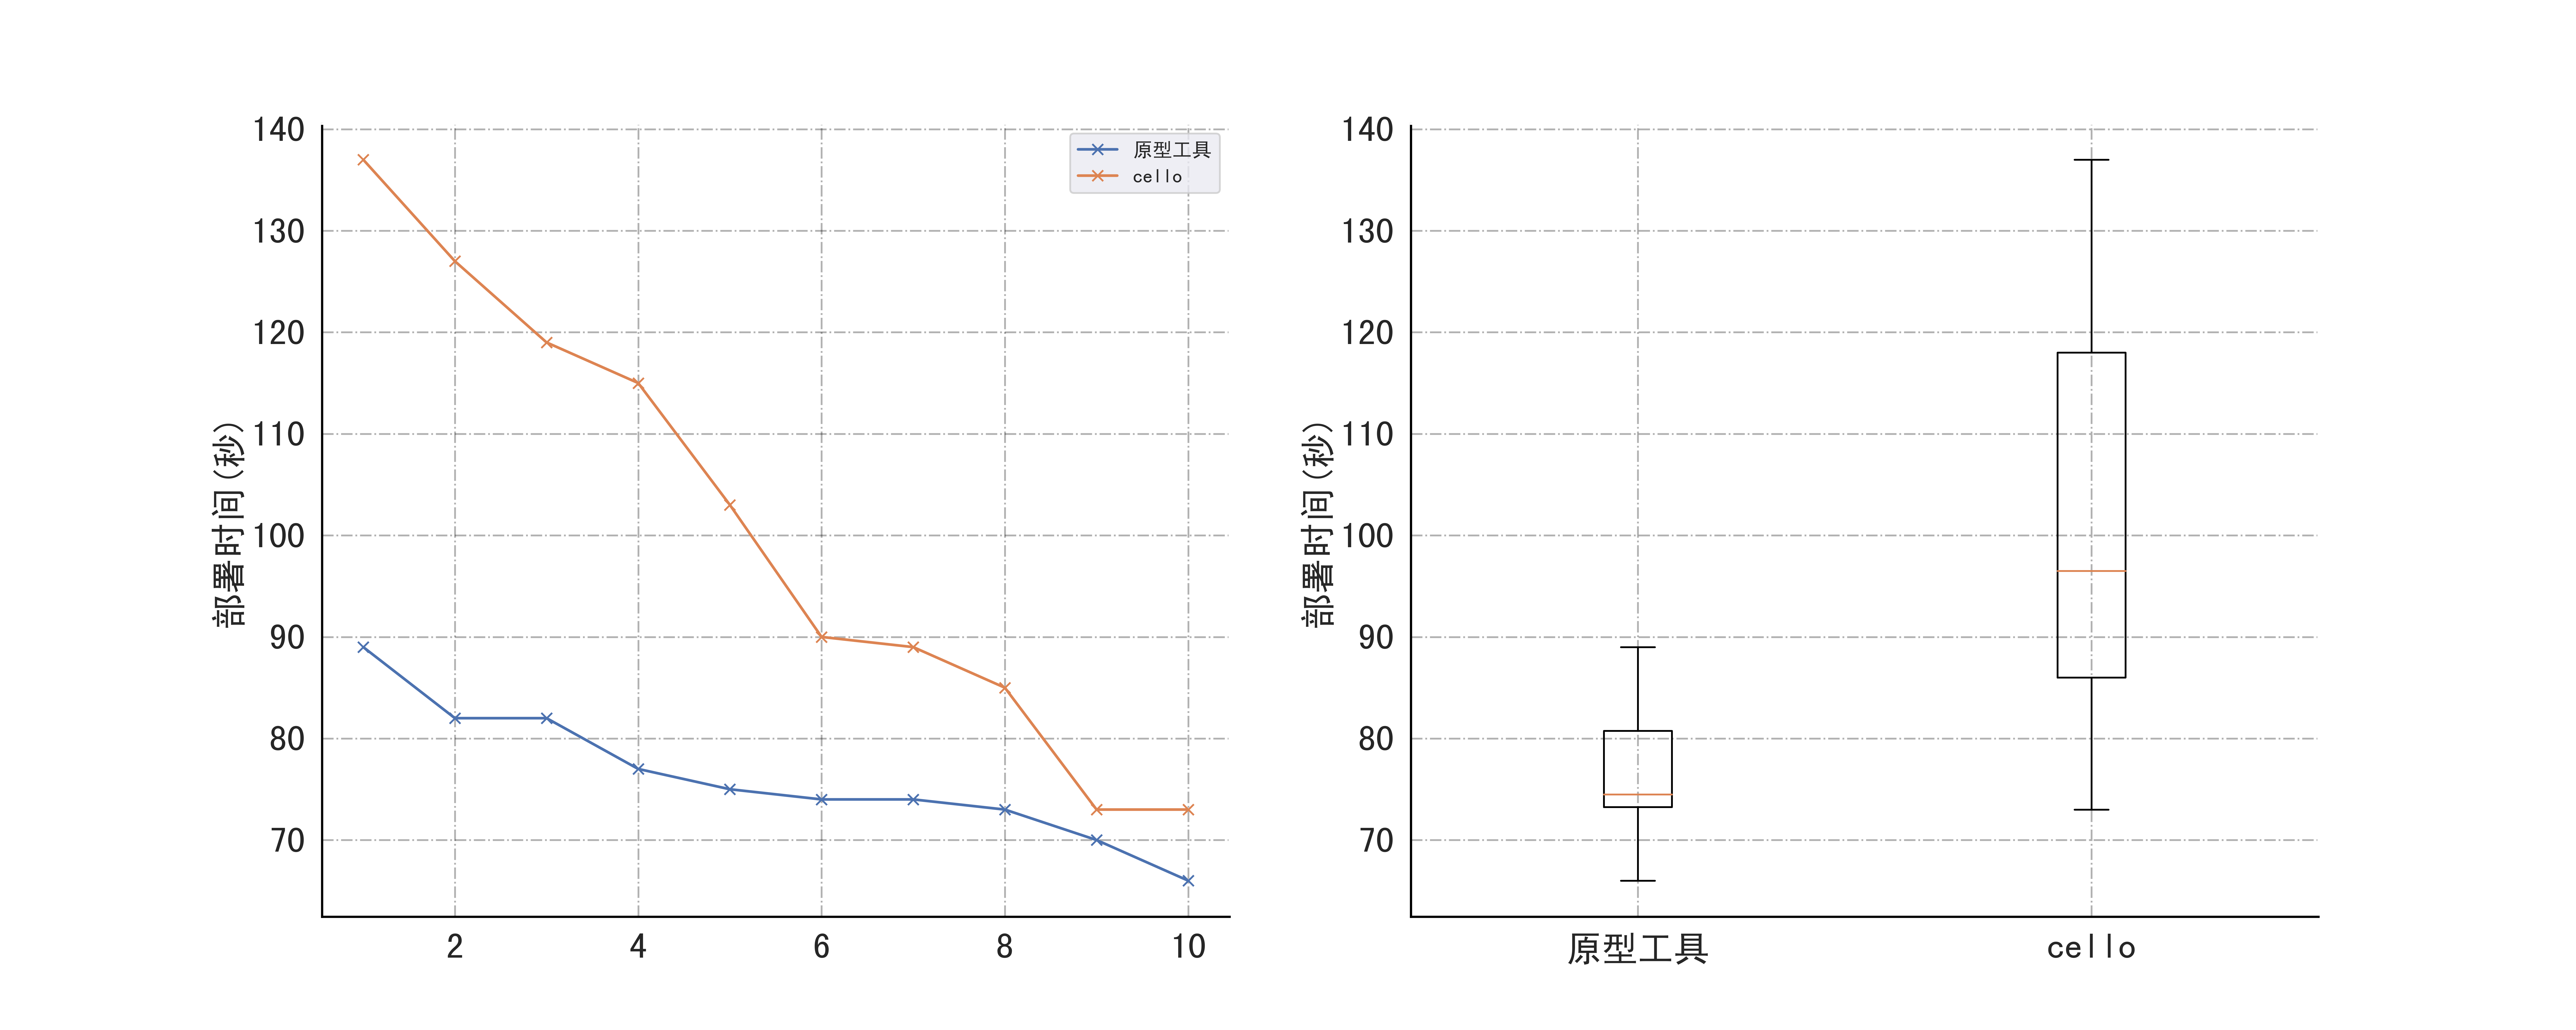
\includegraphics[width=1.0\textwidth]{FIGs/chapter5/plt_deployment.png} %中括号中的参数是设置图片充满文档的大小,你也可以使用小数来缩小图片的尺寸。
    \caption{网络部署时间对比图} %caption是用来给图片加上图题的
    \label{plt_deployment} %这是添加标签,方便在文章中引用图片。
\end{figure}%figure环境

通过分析源码\footnotemark[1]\footnotetext[1]{\href{https://github.com/hyperledger/cello/blob/release-0.9.0-h3c/src/modules/blockchain_network.py}{cello create network}}可知, 当在Cello Operator前端中提交网络之后, Cello对应的Docker Agent会循环解析传入的HF网络节点信息及数量的数据结构, 解析完成后串行构建HF网络中的各类节点。构建过程中, 采用生成Docker Compose文件并启动对应的网络节点。同样, 在部署Kubernetes时根据Template模板在代码中硬编码生成yaml文件。由此可得, Cello网络部署时间会随着HF网络中节点数量的增加而递增。本文的原型工具, 因需要手动以命令的方式部署单个对应网络节点, 其部署时间也会随着节点数量增加而递增。因此, 只对单Orderer单Peer进行对比测试即可预估出不同网络规模下的网络部署时间。

综上, 通过定量分析, 本文原型工具相较于Cello在具有更优的部署时间, 并且每次部署时间更加稳定。

% 链码调用时间
% 数据落盘时间
% 数据读取能力

\section{本章小结}

本章介绍了对原型工具的测试与评估。首先介绍了本文涉及到的两个测试环境, 并以典型案例的方式对原型工具进行了功能性与非功能性测试, 最终的测试符合预期。其次, 本章利用定性与定量的方法, 分别对原型工具进行了评估。最终原型工具基本满足五层成熟度模型, 且原型工具相较于Cello在网络部署时间上更优且更稳定。
